%%%%%%%%%%%%%%%%%%%%%%%%%%%%%%%%%%%%%%%%%%%%%%%%%%%%%%%%%%% Author - Varad Meru
%% tex source file for ML Homeworks
%%%%%%%%%%%%%%%%%%%%%%%%%%%%%%%%%%%%%%%%%%%%%%%%%%%%%%%%%
\documentclass[a4paper, 11pt]{article}

\usepackage[margin=1in]{geometry} % changes the margin
\usepackage{lipsum} % adds random text to check the formatting
\usepackage{hyperref} % adds hyperlink
\usepackage[framed,numbered,autolinebreaks,useliterate]{mcode}
\usepackage{subfigure}
\usepackage{amsmath}
\usepackage{graphicx}
\usepackage{pythonhighlight}
\usepackage{enumerate}

\renewcommand{\thefootnote}{\fnsymbol{footnote}} % Changes the format of the footnotes superscripts

%%%%%%%%%%%%%%%%%%%%%%%%%%%%%%%%%%%%%%%%%%%%%%%%%%%%%%%%%
\begin{document}

\begin{noindent}
\large\textbf{Week 4} \hfill \textbf{Varad Meru} \\
\normalsize CS 273a - Introduction to Machine Learning (Winter '15)\footnote{\href{http://sli.ics.uci.edu/Classes/2015W-273a}{Website: http://sli.ics.uci.edu/Classes/2015W-273a}} \hfill Student \# 26648958 \\
Prof. Alex Ihler \hfill Due Date: 02/24/2015
\end{noindent}	
\noindent\makebox[\linewidth]{\rule{\textwidth}{0.4pt}}

%%%%%%%%%%%%%%%%%%%%%%%%%%%%%%%%%%%%%%%%%%%%%%%%%%%%%%%%%
%%%%%%%%%%%%%%%%%%%%%%%%%%%%%%%%%%%%%%%%%%%%%%%%%%%%%%%%%
\begin{center}
\textbf{\Large{Homework 4}\footnote{Questions available at \href{http://sli.ics.uci.edu/Classes/2015W-273a?action=download\&upname=HW4.pdf}{http://sli.ics.uci.edu/Classes/2015W-273a?action=download\&upname=HW4.pdf}}\footnote{All the figures and listing numbers are auto-referred.}}\\
\end{center}
\vspace{-25pt}

%%%%%%%%%%%%%%%%%%%%%%%%%%%%%%%%%%%%%%%%%%%%%%%%%%%%%%%%%
%%%%%%%%%%%%%%%%%%%%%%%%%%%%%%%%%%%%%%%%%%%%%%%%%%%%%%%%%
%%%%%%%%%%%%%%%%%%%%%%%%%%%%%%%%%%%%%%%%%%%%%%%%%%%%%%%%%
\section*{Problem 1: Support Vector Machines}
The problem of SVM can be solved using two methods - using the Primal Form and the Dual Form. The following describe both approaches to solve the problem of finding the best fit line for the Iris dataset with two classes.

\subsection*{Primal Form}
The code for computing the SVM margins using the Primal form is given in \autoref{lst:primalform}. The generated weights are also given at the end of the listing. The classification can be seen in the \autoref{fig:primalplots}.
\vspace{-20pt}
\begin{lstlisting}[caption={SVM Primal Form},label={lst:primalform},numbers=left,escapeinside={@}{@}]
iris=load('data/iris.txt');     % load the text file
X = iris(:,1:2);       % features are other columns
Y = iris(:,end);           % target value is last column
XA = X(Y<2,:);
YA=Y(Y<2);       % get class 0 vs 1
YB(YA == 0) = -1;
YB(YA == 1) = 1;

XA_CLASS_0 = XA(find(YB==-1),:); %For Class plotting
XA_CLASS_1 = XA(find(YB==1),:);

% Setting the parameters to be given to quadprog
numOfExamples = size(XA,1);
numOfAttributes = size(XA,2);
H = eye( numOfAttributes + 1);
H(numOfAttributes+1,numOfAttributes+1)=0;
f=zeros(numOfAttributes+1,1);

Z = [XA ones(numOfExamples,1)];
A=-diag(YB)*Z;
c=-1*ones(numOfExamples,1);
w=quadprog(H,f,A,c);

% Weights computed by quadprog
learner = logisticClassify2();
learner=setClasses(learner, unique(YA));
wts =[w(3,1) w(1,1) w(2,1)];
learner=setWeights(learner, wts);

yte = predict(learner,XA);
error = errorTrain(YA,yte);

Y1=-(wts(:,2)*XA+wts(:,1))/wts(:,3);  %Seperating hyperplane
YLOW=(-1-wts(:,2)*XA-wts(:,1))/wts(:,3); %Margin
YUP=(1-wts(:,2)*XA-wts(:,1))/wts(:,3); %Margin

% Plots --- 
h = figure;
hold on;
plot(XA_CLASS_0(:,1),XA_CLASS_0(:,2),'or');
plot(XA_CLASS_1(:,1),XA_CLASS_1(:,2),'+b');
hold off;
saveas(h,'primal1.jpg','jpg');

h = figure;
axis([4,7,1.5,5])
hold on;
plot(XA_CLASS_0(:,1),XA_CLASS_0(:,2),'or');
plot(XA_CLASS_1(:,1),XA_CLASS_1(:,2),'+b');
% Plotting the SVM generated decision boundary and margins here!
plot(XA,Y1,'k-');
plot(XA,YUP,'m:');
plot(XA,YLOW,'m:');
hold off;

% Using the  Functions given by Prof. Alex. 
h=figure;
plot2DLinear(learner,XA,YA);
saveas(h,'primal4.jpg','jpg');
h=figure;
plotClassify2D(learner, XA, YA);
saveas(h,'primal3.jpg','jpg');

%{
w =
    6.3572
   -5.3693
  -17.2697
%}

\end{lstlisting}

\begin{figure}
\centering
\subfigure[Scatter plot of Data, with Classes]{
    \label{fig:subfig1}
    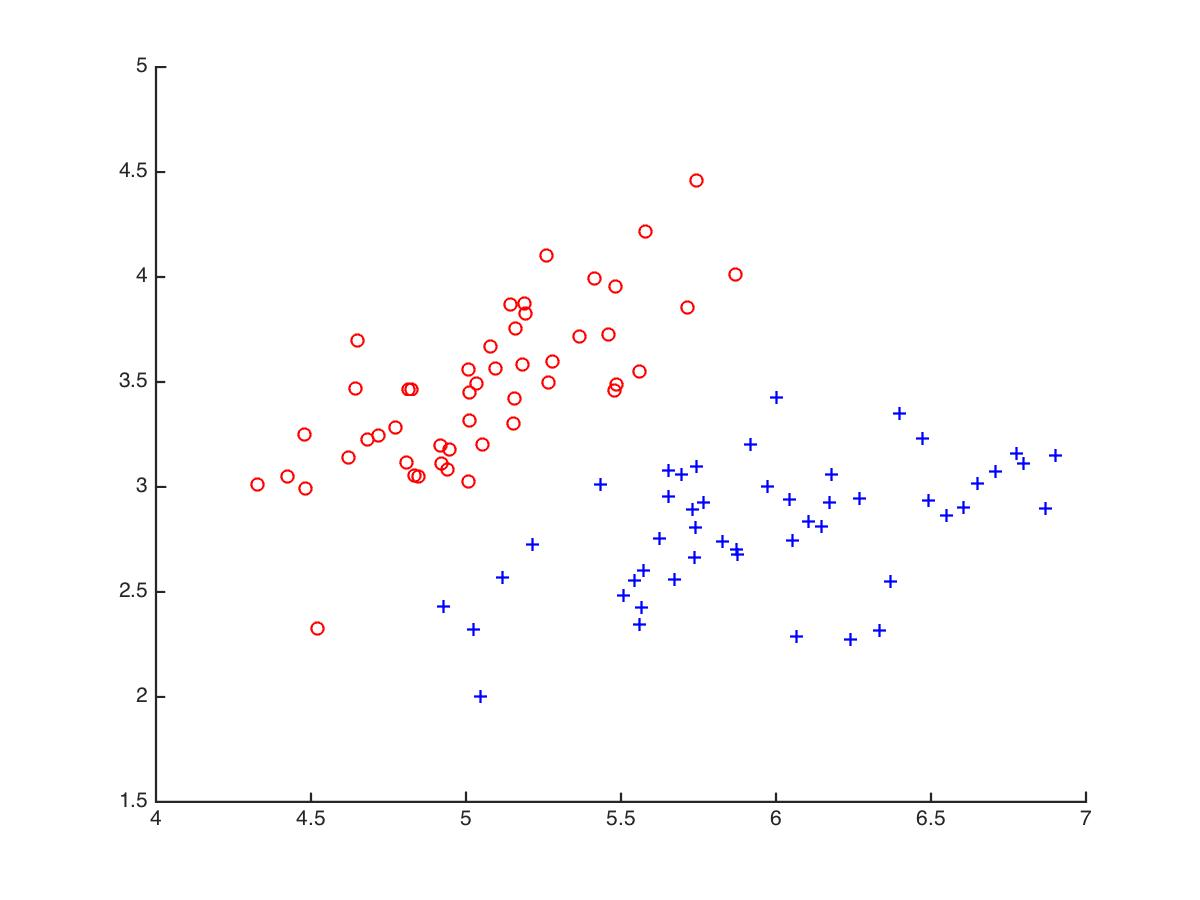
\includegraphics[scale=0.180]{primal1.jpg}
}
\subfigure[The SVM generated Decision Boundary and the Margins]{
    \label{fig:subfig2}
    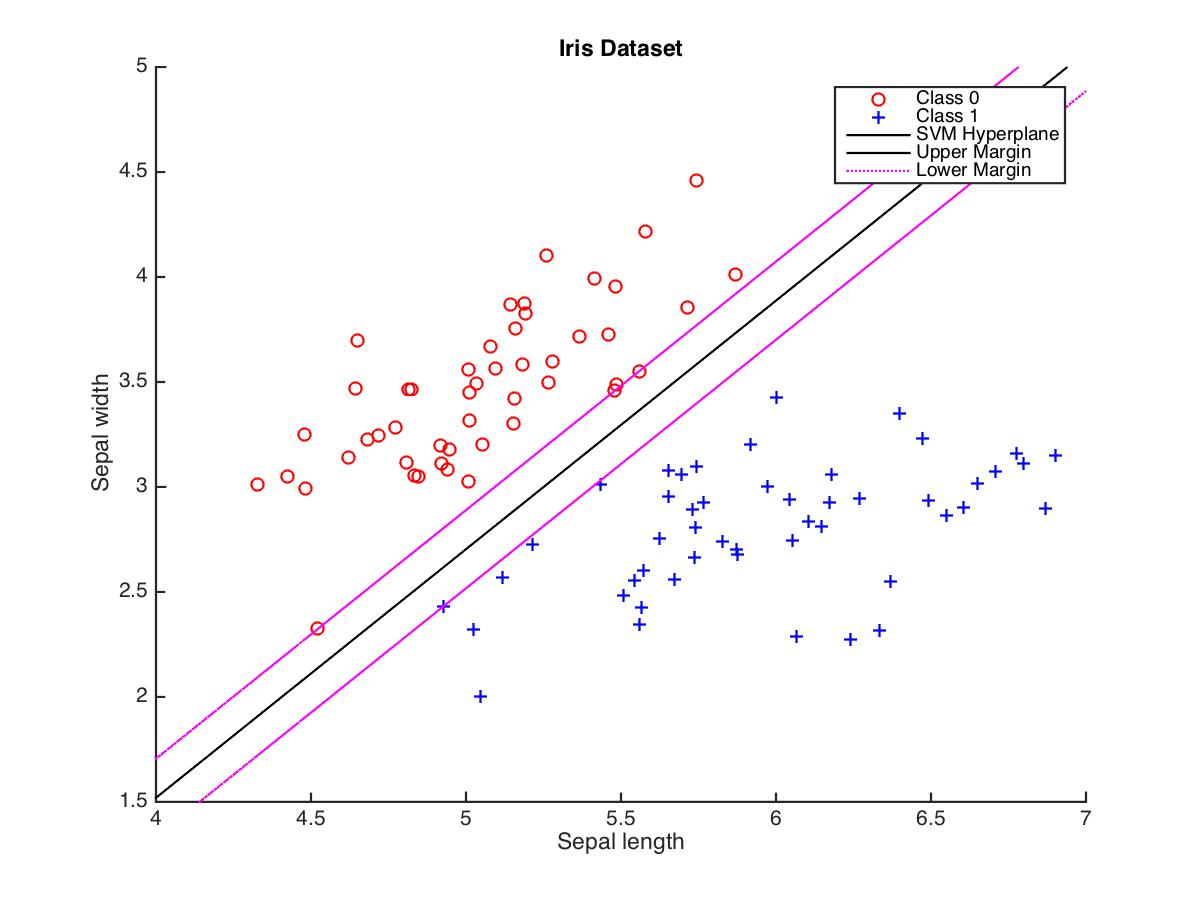
\includegraphics[scale=0.180]{primal2.jpg}
}
\subfigure[The SVM generated Decision Boundary]{
    \label{fig:subfig3}
    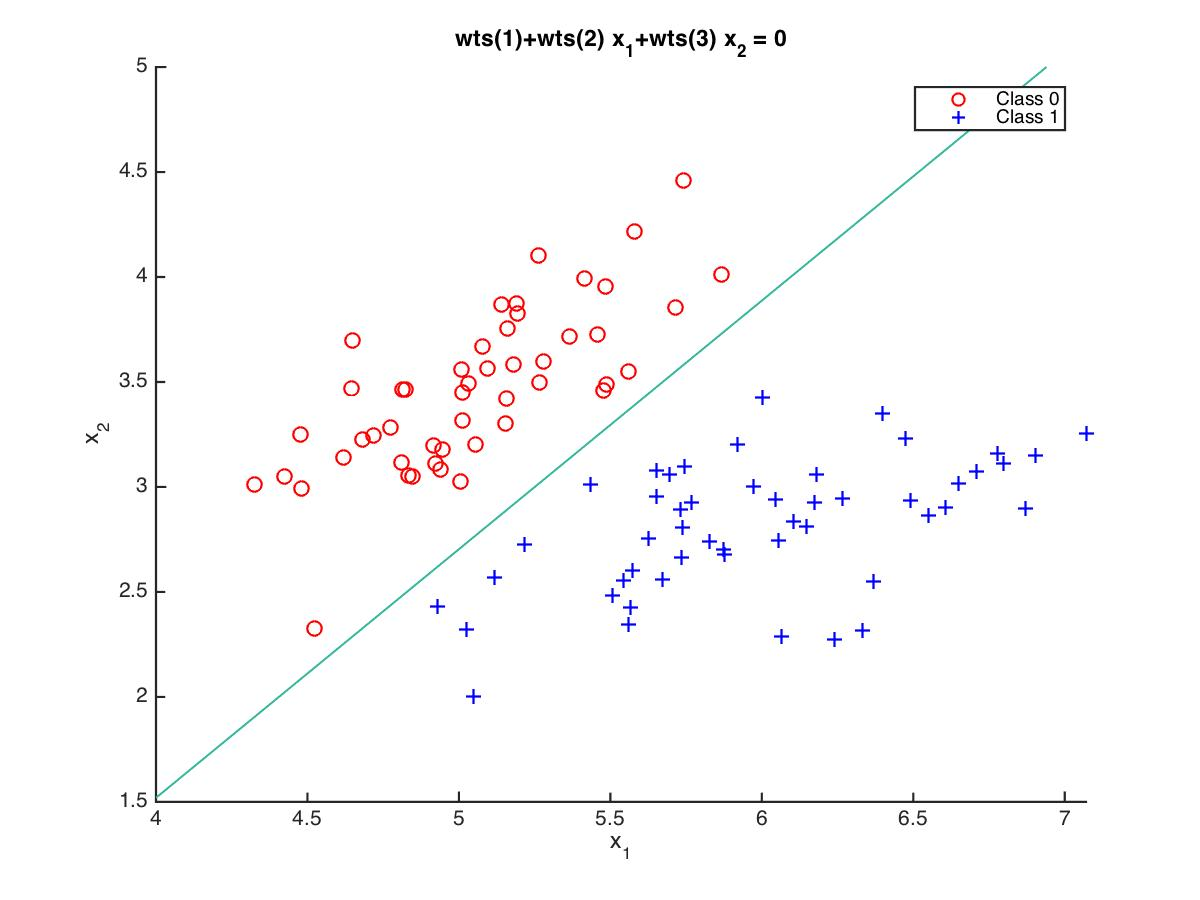
\includegraphics[scale=0.19]{primal4.jpg}
}
\subfigure[The Classification Regions generated by the \mcode{plotClassify2D} function]{
    \label{fig:subfig4}
    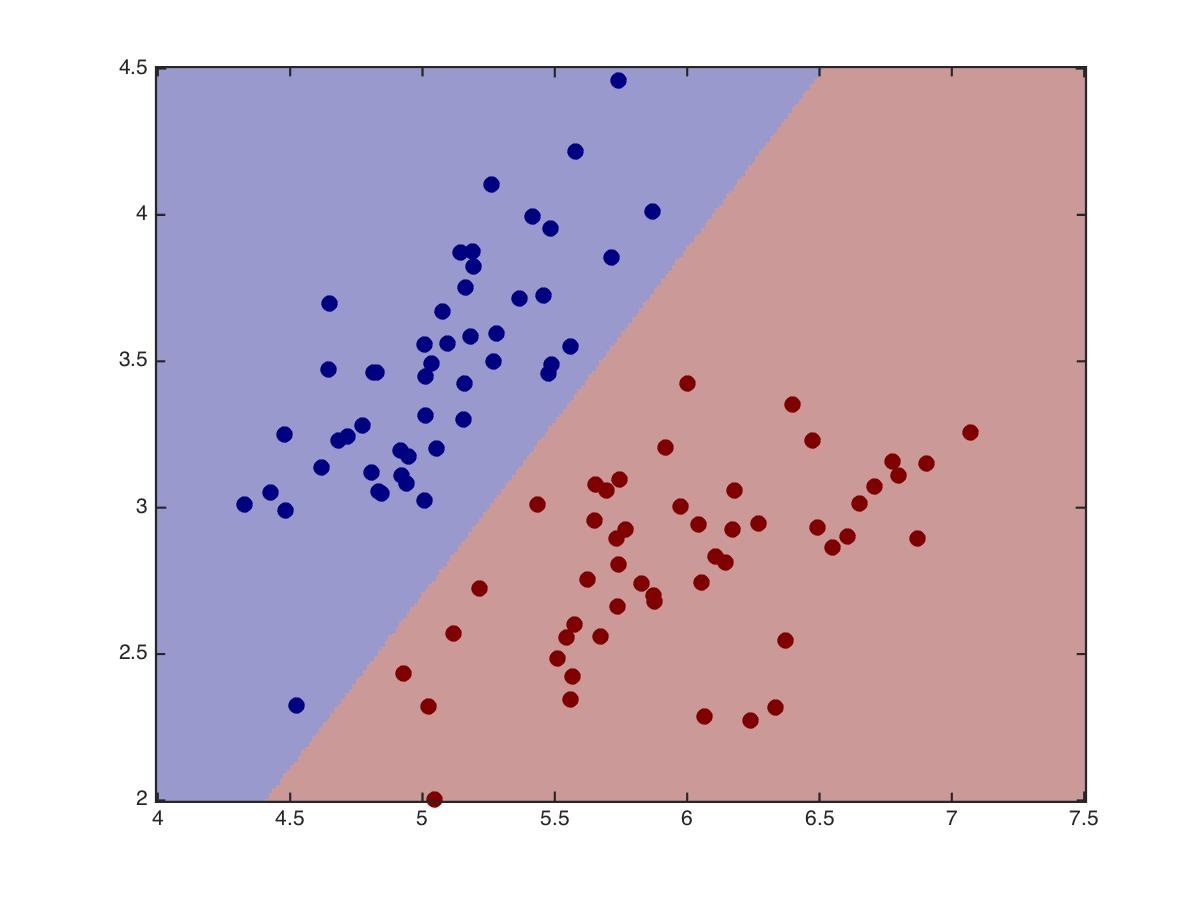
\includegraphics[scale=0.19]{primal3.jpg}
}
\caption[]{The Margins and the Decision Boundary generated using the \textbf{Primal Form} of SVM computation. The figure \autoref{fig:subfig4} uses a different axis scale to plot the classes and may look a little different, with a different slope, but is generated from the same learner.}
\label{fig:primalplots}
\end{figure}

\subsection*{Dual Form}
The code for computing the SVM margins using the Dual form is given in \autoref{lst:dualform}. The generated weights are also given at the end of the listing. The classification can be seen in the \autoref{fig:dualplots}.

\vspace{-20pt}
\begin{lstlisting}[caption={SVM Primal Form},label={lst:dualform},numbers=left,escapeinside={@}{@}]
% Setting the parameters to be given to quadprog
numOfExamples = size(XA,1);
numOfAttributes = size(XA,2);
K = (XA*XA');
H = K .* (YA*YA');
f = -ones(numOfExamples,1);

A = -eye(numOfExamples);
B = zeros(numOfExamples,1);

Aeq = [YA' ; zeros(numOfExamples-1,numOfExamples)];
beq = zeros(numOfExamples,1);
alpha = quadprog(H+eye(numOfExamples)*0.001,f,A,B,Aeq,beq);

% Weights computed by quadprog
w = (alpha.*YA)'*XA;
XSuppVectors = XA(alpha>0.1,:);
YSuppVectors = YA(alpha>0.1);

b = (1/YSuppVectors(1)) - w*XSuppVectors(1,:)';
theta = [b,w];
learner=logisticClassify(); 
learner=setClasses(learner, unique(YA)); 
wts = [b,w];
learner=setWeights(learner, wts); 

h = figure;
plotClassify2D(learner, XA, YA);

%{
    wts =
  -16.7391    6.1716   -5.2282
%}

\end{lstlisting}

\begin{figure}
\centering
\subfigure[Scatter plot of Data, with Classes]{
    \label{fig:subfig5}
    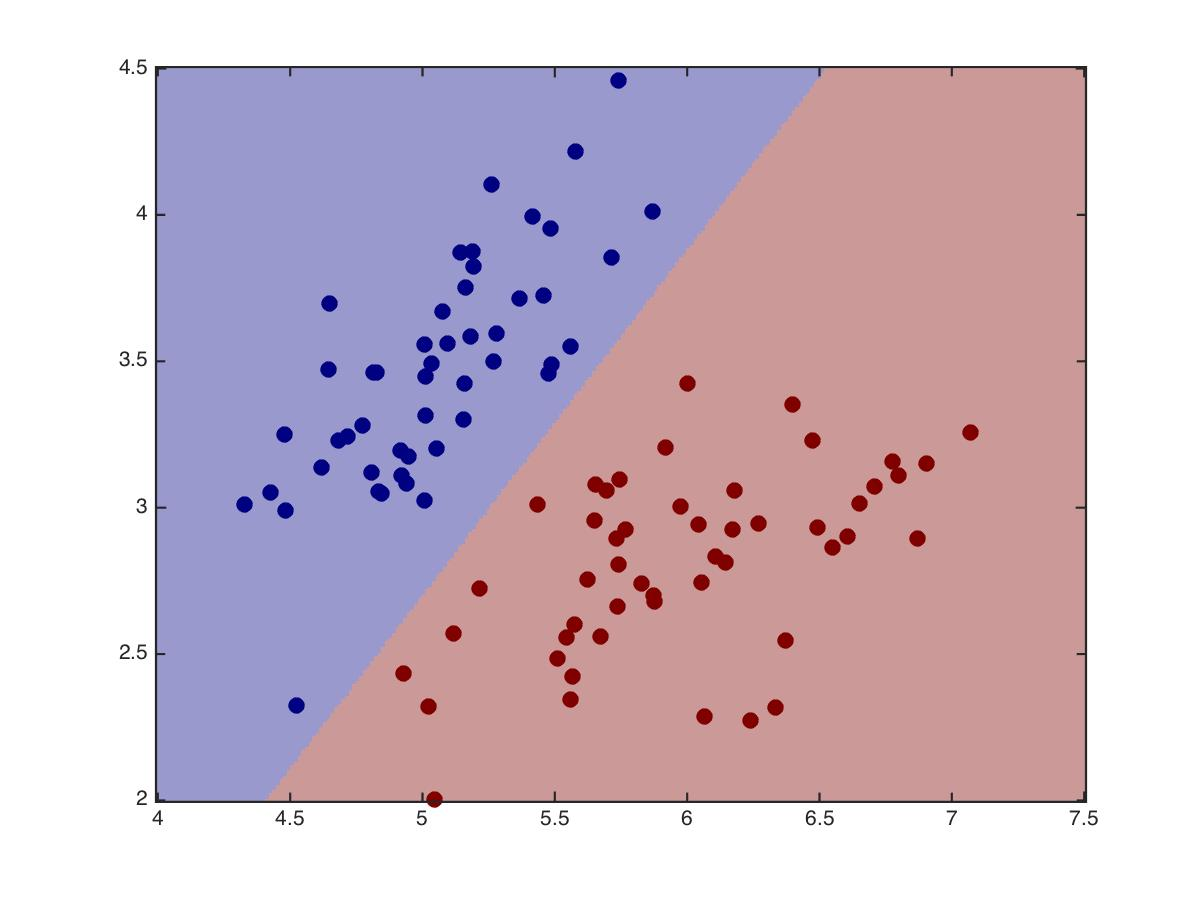
\includegraphics[scale=0.21]{dual.jpg}
}
\subfigure[The SVM generated Decision Boundary and the Margins]{
    \label{fig:subfig6}
    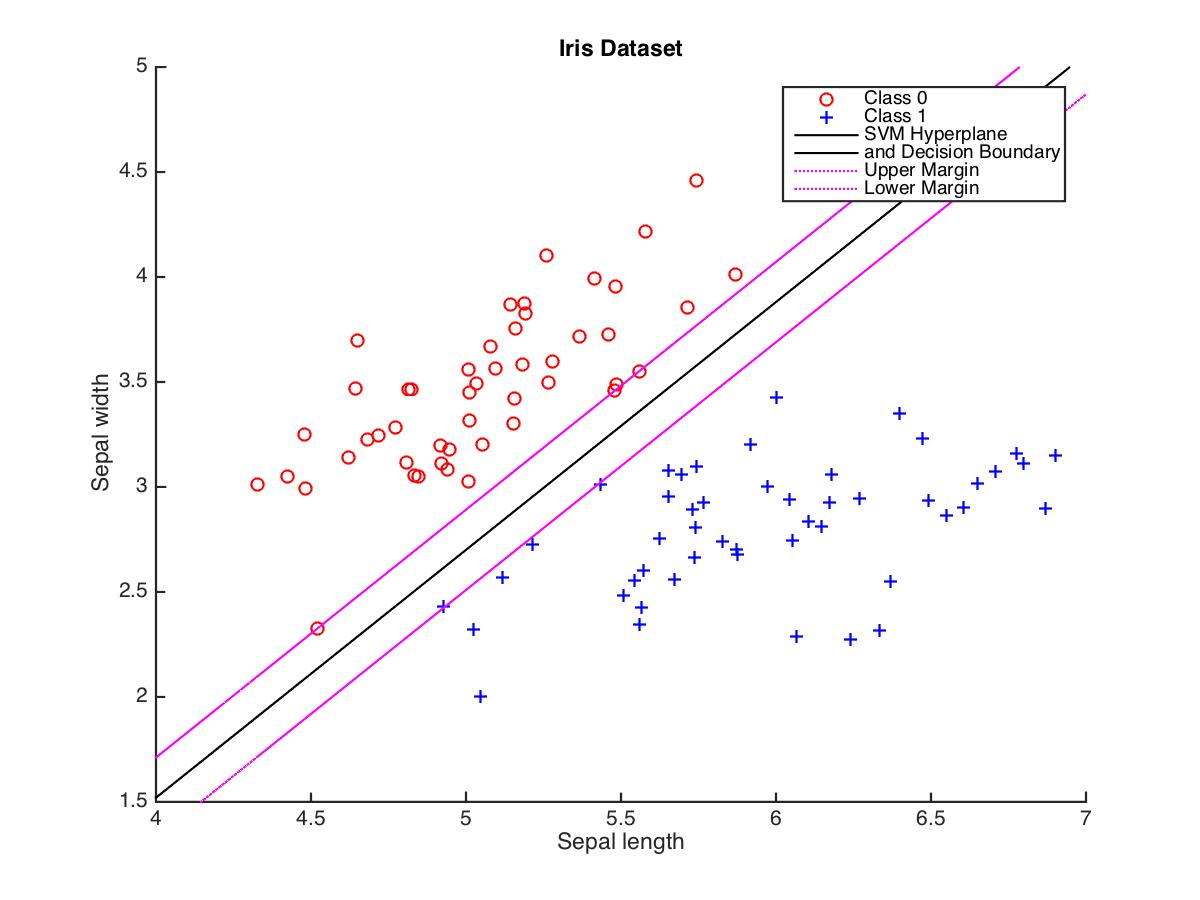
\includegraphics[scale=0.21]{dual2.jpg}
}
\caption[]{The Margins and the Decision Boundary generated using the \textbf{Dual Form} of SVM computation. The figure \autoref{fig:subfig6} uses a different axis scale to plot the classes and may look a little different, with a different slope, but is generated from the same learner.}
\label{fig:dualplots}
\end{figure}

\vspace{-10pt}

%%%%%%%%%%%%%%%%%%%%%%%%%%%%%%%%%%%%%%%%%%%%%%%%%%%%%%%%%
%%%%%%%%%%%%%%%%%%%%%%%%%%%%%%%%%%%%%%%%%%%%%%%%%%%%%%%%%
\pagebreak
\section*{Problem 2: Decision Trees}
\begin{enumerate}[(a)]
\item The entropy of the class variable y ca be computed using the expression of Entropy, given by $H(x) = \sum p(x) log_2(1/p(x))$. Now, the class variable, y, can take 2 values - 0 and 1. Thus, the entropy of the class variable is given in \autoref{eqn:entropy1}.
\begin{equation}
H(y) = \sum p(y) log_2(1/p(y))
= \frac{6}{10}log_2 \frac{10}{6} + \frac{4}{10}log_2 \frac{10}{4} = 0.9710
\label{eqn:entropy1}
\end{equation}

\item The information gain for each attribute is computed as follows
\begin{enumerate}
\item[for $\mathbf{x_1}$:] The new entropy after splitting the feature $\mathbf{x_1}$ is given in \autoref{eqn:ig1}.
\begin{equation}
\label{eqn:ig1}
\begin{split}
H(x_1 = 0) = \frac{3}{4}log_2 \frac{4}{3} + \frac{1}{4}log_2 \frac{4}{1} = 0.8113\text{ bits }\\
H(x_1 = 1) = \frac{3}{6}log_2 \frac{6}{3} + \frac{3}{6}log_2 \frac{6}{3} = 1\text{ bit }
\end{split}
\end{equation}
The expected new entropy is $H(y_{x_1}) = \frac{4}{10} H(x_1 = 0) + \frac{6}{10} H(x_1 = 1) = \frac{4}{10} * 0.8113 + \frac{6}{10} * 1 = 0.9245 bits $

\item[for $\mathbf{x_2}$:] The new entropy after splitting the feature $\mathbf{x_2}$ is given in \autoref{eqn:ig2}.
\begin{equation}
\begin{split}
H(x_2 = 0) = \frac{1}{5}log_2 \frac{5}{1} + \frac{4}{5}log_2 \frac{5}{4} = 0.7219\text{ bits }\\
H(x_2 = 1) = \frac{5}{5}log_2 \frac{5}{5} + \frac{0}{5}log_2 \frac{5}{0} = 0 \text{ bits }
\end{split}
\label{eqn:ig2}
\end{equation}
The expected new entropy is $H(y_{x_2}) = \frac{5}{10} H(x_2 = 0) + \frac{5}{10} H(x_2 = 1) = \frac{5}{10} * 0.7219 + \frac{5}{10} * 0 = 0.3609 bits $

\item[for $\mathbf{x_3}$:] The new entropy after splitting the feature $\mathbf{x_3}$ is given in \autoref{eqn:ig3}.
\begin{equation}
\begin{split}
H(x_3 = 0) = \frac{2}{3}log_2 \frac{3}{2} + \frac{1}{3}log_2 \frac{3}{1} = 0.9183\text{ bits }\\
H(x_3 = 1) = \frac{4}{7}log_2 \frac{7}{4} + \frac{3}{7}log_2 \frac{7}{3} = 0.9852\text{ bits }
\end{split}
\label{eqn:ig3}
\end{equation}
The expected new entropy is $H(y_{x_3}) = \frac{3}{10} H(x_3 = 0) + \frac{7}{10} H(x_3 = 1) = \frac{3}{10} * 0.9183 + \frac{7}{10} * 0.9852 = 0.9651 bits $

\item[for $\mathbf{x_4}$:] The new entropy after splitting the feature $\mathbf{x_4}$ is given in \autoref{eqn:ig4}.
\begin{equation}
\begin{split}
H(x_4 = 0) = \frac{5}{7}log_2 \frac{7}{5} + \frac{2}{7}log_2 \frac{7}{2} = 0.8631\text{ bits }\\
H(x_4 = 1) = \frac{1}{3}log_2 \frac{3}{1} + \frac{2}{3}log_2 \frac{3}{2}  = 0.9183\text{ bits }
\end{split}
\label{eqn:ig4}
\end{equation}
The expected new entropy is $H(y_{x_4}) = \frac{7}{10} H(x_4 = 0) + \frac{3}{10} H(x_4 = 1) = \frac{7}{10} * 0.8631 + \frac{3}{10} * 0.9183 = 0.8797 bits $

\item[for $\mathbf{x_5}$:] The new entropy after splitting the feature $\mathbf{x_5}$ is given in \autoref{eqn:ig5}.
\begin{equation}
\begin{split}
H(x_5 = 0) = \frac{2}{3}log_2 \frac{3}{2} + \frac{1}{3}log_2 \frac{3}{1} = 0.9183\text{ bits }\\
H(x_5 = 1) = \frac{4}{7}log_2 \frac{7}{4} + \frac{3}{7}log_2 \frac{7}{3} = 0.9852\text{ bits }
\end{split}
\label{eqn:ig5}
\end{equation}
The expected new entropy is $H(y_{x_5}) = \frac{3}{10} H(x_5 = 0) + \frac{7}{10} H(x_5 = 1) = \frac{3}{10} * 0.9183 + \frac{7}{10} * 0.9852 = 0.9651 bits $
\end{enumerate}

The information gain for all the features is computed as the difference of the entropy of the class variables without splitting and the expected new entropy after splitting. The entropy of the class variable is calculated in the part (a) of the question ($H(y) = 0.9710$).
\begin{enumerate}
\item[for $x_1$:] $ H(y) - H(y_{x_1}) = 0.9710 - 0.9245 = 0.0465 \text{ bits } $
\item[for $x_2$:] $ H(y) - H(y_{x_2}) = 0.9710 - 0.3609 = 0.6101 \text{ bits } $ 
\item[for $x_3$:] $ H(y) - H(y_{x_3}) = 0.9710 - 0.9651 = 0.0059 \text{ bits } $
\item[for $x_4$:] $ H(y) - H(y_{x_4}) = 0.9710 - 0.8797 = 0.0913 \text{ bits } $
\item[for $x_5$:] $ H(y) - H(y_{x_5}) = 0.9710 - 0.9651 = 0.0059 \text{ bits } $
\\
\\
As splitting x2 gives the most gain, it is better to split on feature $\mathbf{x_2}$ first.
\end{enumerate}

\item I created the decision tree using the \pyth{scikit-learn.tree} package. The learned decision tree is plotted at \autoref{fig:emailtree}. In the displayed tree, the components X[i] correspond to input features as follows:
\begin{itemize}
\item[] X[0] - Feature $\mathbf{x_1}$ - know author? 0: No, 1: Yes
\item[] X[1] - Feature $\mathbf{x_2}$ - is long? 0: No, 1: Yes
\item[] X[2] - Feature $\mathbf{x_3}$ - has 'research'? 0: No, 1: Yes
\item[] X[3] - Feature $\mathbf{x_4}$ - has 'grade'? 0: No, 1: Yes
\item[] X[4] - Feature $\mathbf{x_5}$ - has 'lottery'? 0: No, 1: Yes
\end{itemize}

The information gain is also completed using two custom functions displayed in \autoref{fig:pythonsktreeinfogain} and the output is at \autoref{fig:pythonsktreeinfogain1}

\begin{figure}
\begin{python}[caption={SVM Primal Form},label={lst:pythonsktree}]
from sklearn import tree
import pandas as pd
import numpy as np
import matplotlib.pyplot as plt
import StringIO
import pydot
from IPython.display import Image

email_dict = {'x1' : [0., 1., 0., 1., 0., 1., 0., 1., 1., 1.],
     'x2' : [0., 1., 1., 1., 1., 0., 0., 0., 0., 1.],
     'x3' : [1., 0., 1., 1., 0., 1., 1., 0., 1., 1.],
     'x4' : [1., 1., 1., 1., 0., 1., 0., 0., 1., 1.],
     'x5' : [0., 0., 1., 0., 0., 1., 0., 0., 0., 1.],
     'y' : [-1., -1., -1., -1., -1., 1., 1., 1., 1., -1.]
     }

df_email = pd.DataFrame(email_dict)
header = list(df_email.columns)
featureList=header[:-1]
X=df_email[featureList].values
y=df_email[header[-1]].values

clf=tree.DecisionTreeClassifier(criterion="entropy")
clf.fit(X,y)
dot_data = StringIO.StringIO()
tree.export_graphviz(clf, out_file=dot_data)
graph = pydot.graph_from_dot_data(dot_data.getvalue())
graph.write_png("EmailSpamDecisionTree.png")
\end{python}
\caption[]{\pyth{scikit-learn.tree} based implementation to create the train tree and generate a visual tree.}
\label{fig:pythonsktree}
\end{figure}

\begin{figure}
\centering
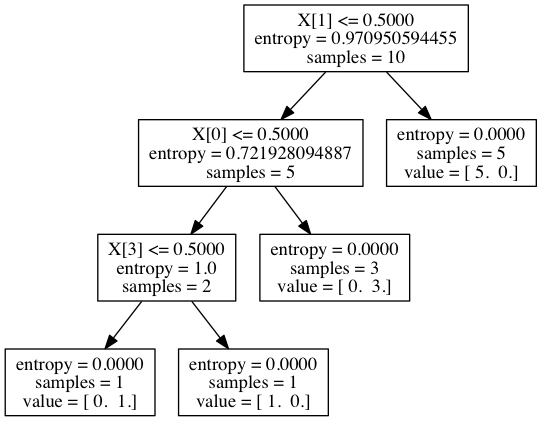
\includegraphics[scale=0.70]{EmailSpamDecisionTree.png}
\caption[]{Email Spam Decision Tree generated by Python code at \autoref{fig:pythonsktree}}
\label{fig:emailtree}
\end{figure}

\begin{figure}
\begin{python}[caption={SVM Primal Form},label={lst:pythonsktree}]
def getEntropy(D):
    """
    Calculate and return entropy of 1-dimensional numpy array D 
    """
    length=D.size
    valueList=list(set(D))
    numVals=len(valueList)
    countVals=np.zeros(numVals)
    Ent=0
    for idx,val in enumerate(valueList):
        countVals[idx]=np.count_nonzero(D==val)
        Ent+=countVals[idx]*1.0/length*np.log2(length*1.0/countVals[idx])
    return Ent 

def getMaxInfoGain(D,X,feat=0):
    """ 
    Calculate maximum information gain w.r.t. the feature which is specified in column feat of the 2-dimensional array X.
    """
    EntWithoutSplit=getEntropy(D)
    feature=X[:,feat]
    length=len(feature)
    valueList=list(set(feature))
    splits=np.diff(valueList)/2.0+valueList[:-1]
    maxGain=0
    bestSplit=0
    bestPart1=[]
    bestPart2=[]
    for split in splits:
        Part1idx=np.argwhere(feature<=split)
        Part2idx=np.argwhere(feature>split)
        E1=getEntropy(D[Part1idx[:,0]])
        l1=len(Part1idx)
        E2=getEntropy(D[Part2idx[:,0]])
        l2=len(Part2idx)
        Gain=EntWithoutSplit-(l1*1.0/length*E1+l2*1.0/length*E2)
        if Gain > maxGain:
            maxGain=Gain
            bestSplit=split
            bestPart1=Part1idx
            bestPart2=Part2idx
    return maxGain,bestSplit,bestPart1,bestPart2
    
print 'Class Labels of entire training dataet: ',y    
E=getEntropy(y)
print "Entropy of Class Labels= ",E
for col in range(X.shape[1]):
    print '-'*30
    print "Best split w.r.t. to feature %s" % header[col]
    maxG,bestSplit,Part1,Part2=getMaxInfoGain(y,X,feat=col)
    print "Maximum Information Gain = ",maxG
    print "Best Split = ",bestSplit
    print "Samples in partition 1: ",len(Part1)
    print "Samples in partition 2: ",len(Part2)
\end{python}
\caption[]{\pyth{scikit-learn} implementation to create the decision tree.}
\label{fig:pythonsktreeinfogain}
\end{figure}

\begin{figure}
\begin{python}[caption={SVM Primal Form},label={lst:pythonsktree}]
'''
Class Labels of entire training dataet:  [-1. -1. -1. -1. -1.  1.  1.  1.  1. -1.]
Entropy of Class Labels=  0.970950594455
------------------------------
Best split w.r.t. to feature x1
Maximum Information Gain =  0.046439344671
Best Split =  0.5
Samples in partition 1:  4
Samples in partition 2:  6
------------------------------
Best split w.r.t. to feature x2
Maximum Information Gain =  0.609986547011
Best Split =  0.5
Samples in partition 1:  5
Samples in partition 2:  5
------------------------------
Best split w.r.t. to feature x3
Maximum Information Gain =  0.00580214901435
Best Split =  0.5
Samples in partition 1:  3
Samples in partition 2:  7
------------------------------
Best split w.r.t. to feature x4
Maximum Information Gain =  0.0912774462417
Best Split =  0.5
Samples in partition 1:  3
Samples in partition 2:  7
------------------------------
Best split w.r.t. to feature x5
Maximum Information Gain =  0.00580214901435
Best Split =  0.5
Samples in partition 1:  7
Samples in partition 2:  3
'''
\end{python}
\caption[]{Information gain computed by the functions displayed at \autoref{fig:pythonsktreeinfogain}}
\label{fig:pythonsktreeinfogain1}
\end{figure}
\end{enumerate}

%%%%%%%%%%%%%%%%%%%%%%%%%%%%%%%%%%%%%%%%%%%%%%%%%%%%%%%%%
%%%%%%%%%%%%%%%%%%%%%%%%%%%%%%%%%%%%%%%%%%%%%%%%%%%%%%%%%
\pagebreak
\section*{Problem 3: Decision Trees on Kaggle}
\begin{enumerate}[(a)]
\item The Validation Data is shuffled and split (75:25) and the \mcode{treeRegress} class is used as the learner on the data. The code that performs this computation can be seen in \autoref{lst:treeregress1}
\vspace{-25pt}
\begin{lstlisting}[caption={Tree Regression on Kaggle competition dataset},label={lst:treeregress1},numbers=left,escapeinside={@}{@}]
% Problem a - Decision trees on Kaggle
X=load('data/kaggle/kaggle.X1.train.txt');     % load the text file
Y=load('data/kaggle/kaggle.Y.train.txt');     % load the text file

[X, Y] = shuffleData(X,Y);
[Xtr, Xte, Ytr, Yte] = splitData(X,Y, .75); % split data into 75/25 train/test

dt = treeRegress(Xtr,Ytr, 'maxDepth',20);
mse(dt,Xte,Yte) 
% ans = 0.7367

dt = treeRegress(Xtr,Ytr, 'maxDepth',15);
mse(dt,Xte,Yte)
% ans = 0.6384
\end{lstlisting}

\item Now for varying \mcode{maxDepth}, the \autoref{lst:treeregress2} produces the \mcode{semilogx} graph of the error function. The \autoref{fig:lr1} shows the error plots for test and training errors. The complexity of the model is increasing as the \mcode{maxDepth} value is increased. Also, I could see the model overfitting, with the test error plots showing that indication. For my shuffle and split dataset, the depth of 7 gives the least test errors, and thus should be the choice.
\vspace{-20pt}
\begin{lstlisting}[caption={Tree Regression on Kaggle competition dataset with varying \mcode{maxDepth}},label={lst:treeregress2},numbers=left,escapeinside={@}{@}]
%% Part b
for f=1:20;
    dt = treeRegress(Xtr,Ytr, 'maxDepth',f);
    errorsTe(f) = mse(dt,Xte,Yte);
    errorsTr(f) = mse(dt,Xtr,Ytr);
end;

K = (1:20);
h=figure;
semilogx(log(K), errorsTr);
hold on;
semilogx(log(K), errorsTe);
saveas(h,'maxdepth.jpg','jpg');
\end{lstlisting}

\begin{figure}
\centering
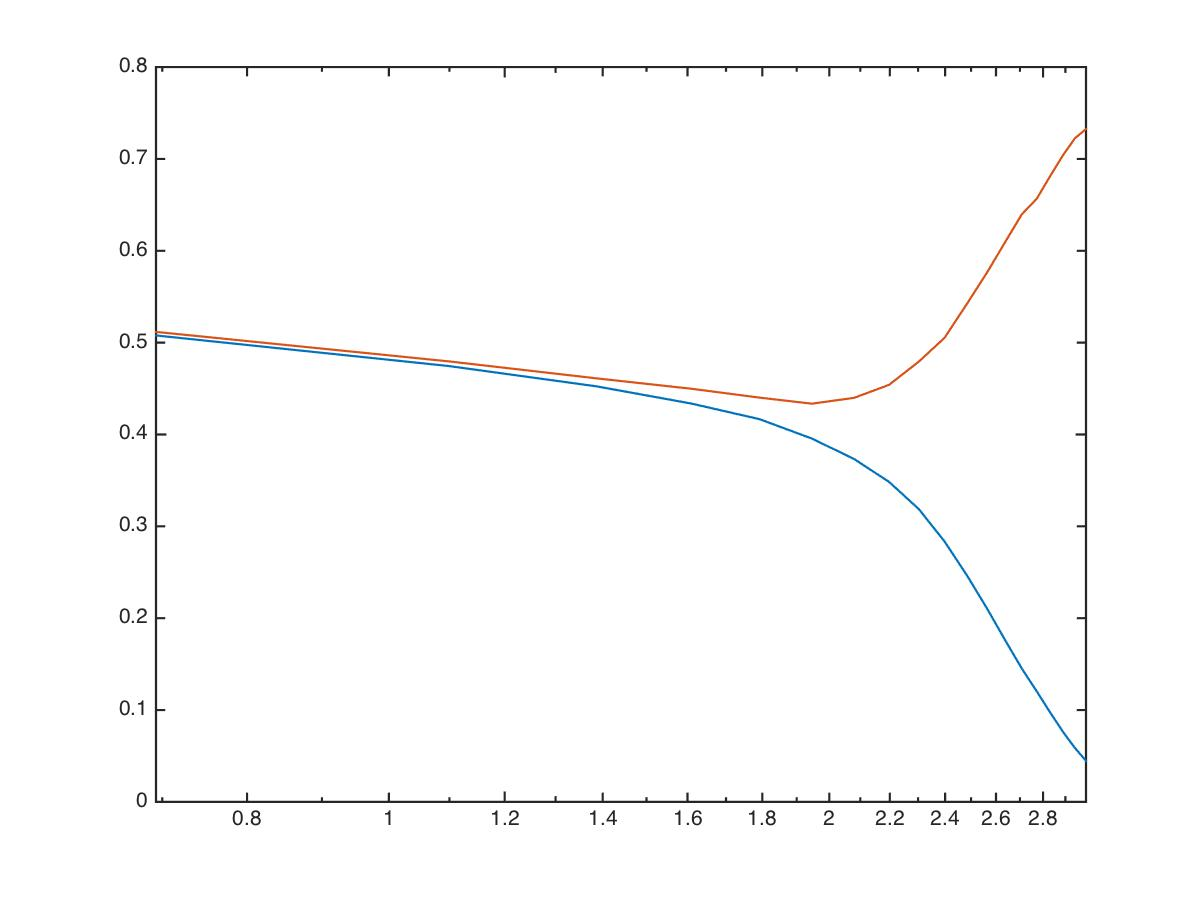
\includegraphics[scale=0.25]{maxdepth.jpg}
\caption[]{For varying values of \mcode{maxDepth}, the Train and Test Error is plotted}
\label{fig:lr1}
\end{figure}

\item Now for varying \mcode{minParent}, the \autoref{lst:treeregress3} produces the \mcode{semilogx} graph of the error function. The \autoref{fig:lr2} shows the error plots for test and training errors. The complexity of the model is increasing as the \mcode{minParent} value is increased. Also, I could see the model overfitting, with the test error plots showing that indication. For my shuffle and split dataset, the depth of 7 gives the least test errors, and thus should be the choice.
\vspace{-20pt}
\begin{lstlisting}[caption={Tree Regression on Kaggle competition dataset with varying \mcode{minParent}},label={lst:treeregress3},numbers=left,escapeinside={@}{@}]
%% Part c
mxDepth = 20;
for f=3:12;
    dt = treeRegress(Xtr,Ytr, 'maxDepth',mxDepth,'minParent',2^f);
    errorsTe1(f) = mse(dt,Xte,Yte);
    errorsTr1(f) = mse(dt,Xtr,Ytr);
end;

K = [3:12];
h=figure;
semilogx(log(K), errorsTr1(:,3:12));
hold on;
semilogx(log(K), errorsTe1(:,3:12));
saveas(h,'minParent.jpg','jpg');
\end{lstlisting}

\begin{figure}
\centering
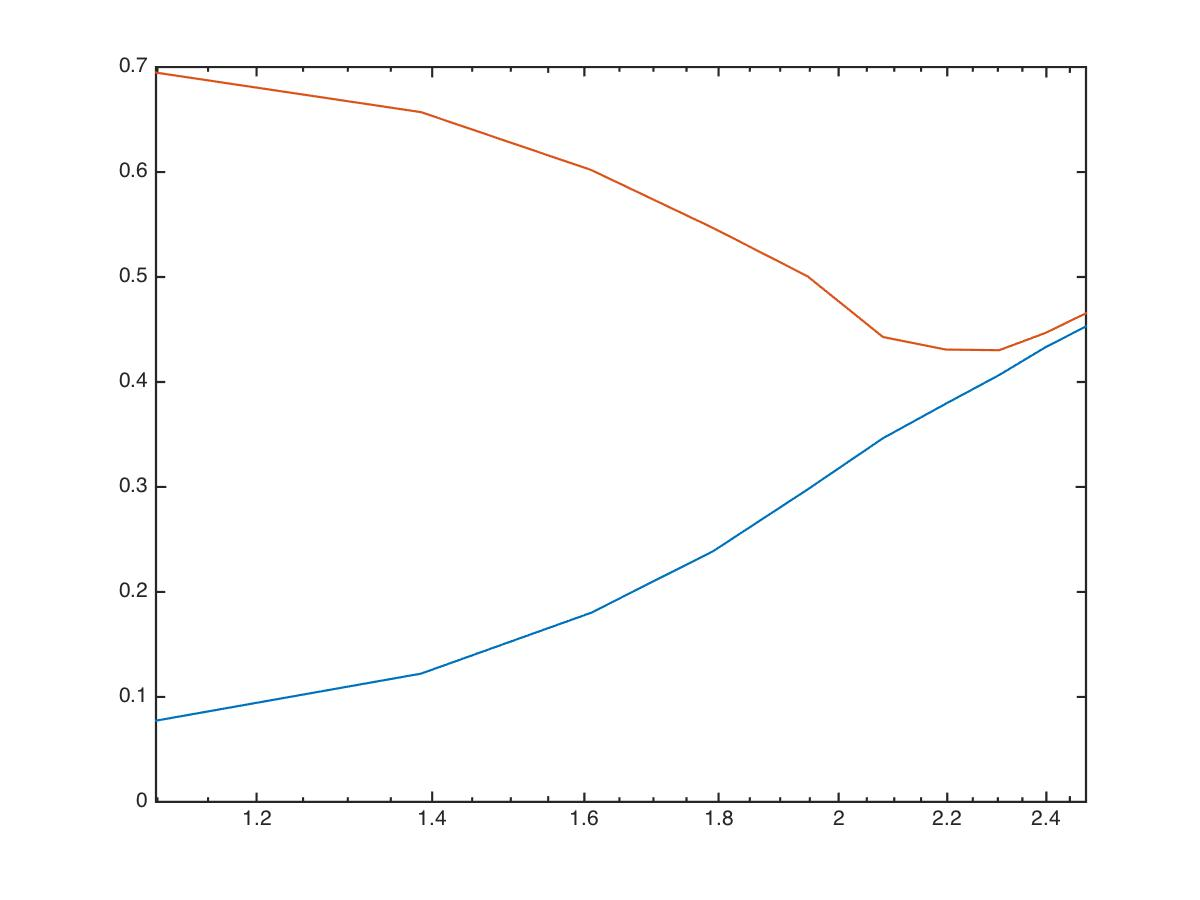
\includegraphics[scale=0.25]{minParent.jpg}
\caption[]{For varying values of \mcode{minParent}, the Train and Test Error is plotted}
\label{fig:lr2}
\end{figure}

\item For the various values of \mcode{minParent} and \mcode{maxParent}, the \autoref{lst:treeregress4} presents the generated output, in comments. The submission on Kaggle.com produced an error of 0.65629 and rank was 141.
\vspace{-20pt}
\begin{lstlisting}[caption={Tree Regression on Kaggle competition dataset for various combinations of maxDepth and minParent},label={lst:treeregress4},numbers=left,escapeinside={@}{@}]
mxDepth = 20;
smallestD = 0;
smallestP = 0;
smallestMSE = 100000;
i = 1;

for d=08:09;
    for p=[350 360 370 380 390 400];
    %for p=[1 10 50 100 150 200 250 300 350 400 450 500 550 600 650 700 750 800 850 900 950 1024];
        dt = treeRegress(Xtr,Ytr, 'maxDepth',d,'minParent',p);
        temp = mse(dt,Xte,Yte);
        disp([temp d p]);
        if temp < smallestMSE
            errors(i,:) = [temp d p];
            disp(errors(i,:));
            smallestMSE = temp;
            smallestD = d;
            smallestP = p;
            i = i+1;
        end
    end;
end;

errors =

    0.5747    1.0000    3.0000
    0.5205    2.0000    3.0000
    0.4863    3.0000    3.0000
    0.4704    4.0000    3.0000
    0.4703    4.0000   10.0000
    0.4601    5.0000    3.0000
    0.4488    6.0000    3.0000
    0.4488    6.0000    5.0000
    0.4383    7.0000    3.0000
    0.4383    7.0000    7.0000
    0.4375    8.0000    8.0000
    Lowest 8 depth , 2^8 minParent
%}

\end{lstlisting}

\end{enumerate}

%%%%%%%%%%%%%%%%%%%%%%%%%%%%%%%%%%%%%%%%%%%%%%%%%%%%%%%%%
%%%%%%%%%%%%%%%%%%%%%%%%%%%%%%%%%%%%%%%%%%%%%%%%%%%%%%%%%
\pagebreak
\section*{Problem 4: Ensembles}
\subsection*{Gradient Boosting}
\begin{enumerate}[(a)]
\item The pseudo-code from the slides is used, but there were some errors in Matlab implementation (given in \autoref{lst:kaggleboosting}). I then looked at \pyth{scikit-learn} for the gradient boosting implementation for large numbers of learner. The code is given in \autoref{fig:boosting1}. This code was tested for a very high number of learner (n=2000) to check if it overfits or not. This test took substantial amount of time but eventually was able to give reasonable results.

\item For n=50, the Kaggle score got improved by 0.01997 from the previous error of 0.65629. The error became 0.63631. And the rank was 138. After n = 2000, the score got improved by  0.03476, with the current accuracy being 0.60155 and the current rank being 11. (Kaggle Username : vrdmr)

\vspace{-15pt}
\begin{lstlisting}[caption={Gradient Boosting in \mcode{MATLAB}},label={lst:kaggleboosting},numbers=left,escapeinside={@}{@}]
%%
dt = treeRegress(Xtr,Ytr, 'maxDepth',20);
mse(dt,Xte,Yte) 
% ans = 0.7367

dt = treeRegress(Xtr,Ytr, 'maxDepth',15);
mse(dt,Xte,Yte)
% ans = 0.6384

%%
% Dataset X,Y
mu = mean(Y); % Often start with constant ?mean? predictor 
dY = Y - mu; % subtract this prediction away
Nboost = 20;
for k=1:Nboost,
  Learner{k} = treeRegress(X,dY, 'maxDepth',15);
  alpha(k) = 1;  % alpha: a ?learning rate? or ?step size?
  % smaller alphas need to use more classifiers, but tend to
  %   predict better given enough of them
  % compute the residual given our new prediction
  dY = dY - alpha(k) * predict(Learner{k}, X);
end;

% Test data Xtest
[Ntest,D] = size(Xeval);
predict = zeros(Ntest,1);      % Allocate space
for k=1:Nboost,                % Predict with each learner
  predict = predict + alpha(k)*predict(Learner{k}, Xeval);
end;
\end{lstlisting}


\begin{figure}
\begin{python}[caption={SVM Primal Form},label={lst:pythonsktree}]
from sklearn.ensemble import GradientBoostingRegressor
from sklearn.cross_validation import train_test_split
from sklearn.metrics import mean_squared_error
from sklearn import tree
import pandas as pd

def boost():
    X = pd.read_csv('../data/kaggle/kaggle.X1.train.txt', header=None)
    Y = pd.read_csv('../data/kaggle/kaggle.Y.train.txt', header=None)
    Xtest = pd.read_csv('../data/kaggle/kaggle.X1.test.txt', header=None)
    Xtr, Xte, Ytr, Yte = train_test_split(X, Y, test_size=0.25, random_state=42)

    est = GradientBoostingRegressor(n_estimators=2000, max_depth=3, min_samples_leaf=300)
    est.fit(Xtr, Ytr)

    pred = est.predict(Xtest)
    pd.Series(pred).to_csv('../data/kaggle/pyprediction.csv', header=['Prediction'], index=True, index_label='ID')
    
boost()
\end{python}
\caption[]{Generating the gradient AdaBooting model using \pyth{scikit-learn}'s ensemble package.}
\label{fig:boosting1}
\end{figure}
\end{enumerate}

\end{document}

%%%%%%%%%%%%%%%%%%%%%%%%%%%%%%%%%%%%%%%%%%%%%%%%%%%%%%%%%
%%%%%%%%%%%%%%%%%%%%%%%That's all folks%%%%%%%%%%%%%%%%%%%%%%%%%%%
%%%%%%%%%%%%%%%%%%%%%%%%%%%%%%%%%%%%%%%%%%%%%%%%%%%%%%%%%
\iffalse
\begin{figure}
\centering
\subfigure[Puzzle 1]{
    \label{fig:subfig1}
    \includegraphics[scale=0.30]{g1.png}
}
\subfigure[Puzzle 2]{
    \label{fig:subfig2}
    \includegraphics[scale=0.30]{g2.png}
}
\caption[Running Various Experiments]{Running Various Experiments. The three bars are for Brute Force, I-Consistency and I-Consistency with MRV search. All the times given are in Seconds}
\label{fig:rungraphs}
\end{figure}

\begin{figure}
\centering
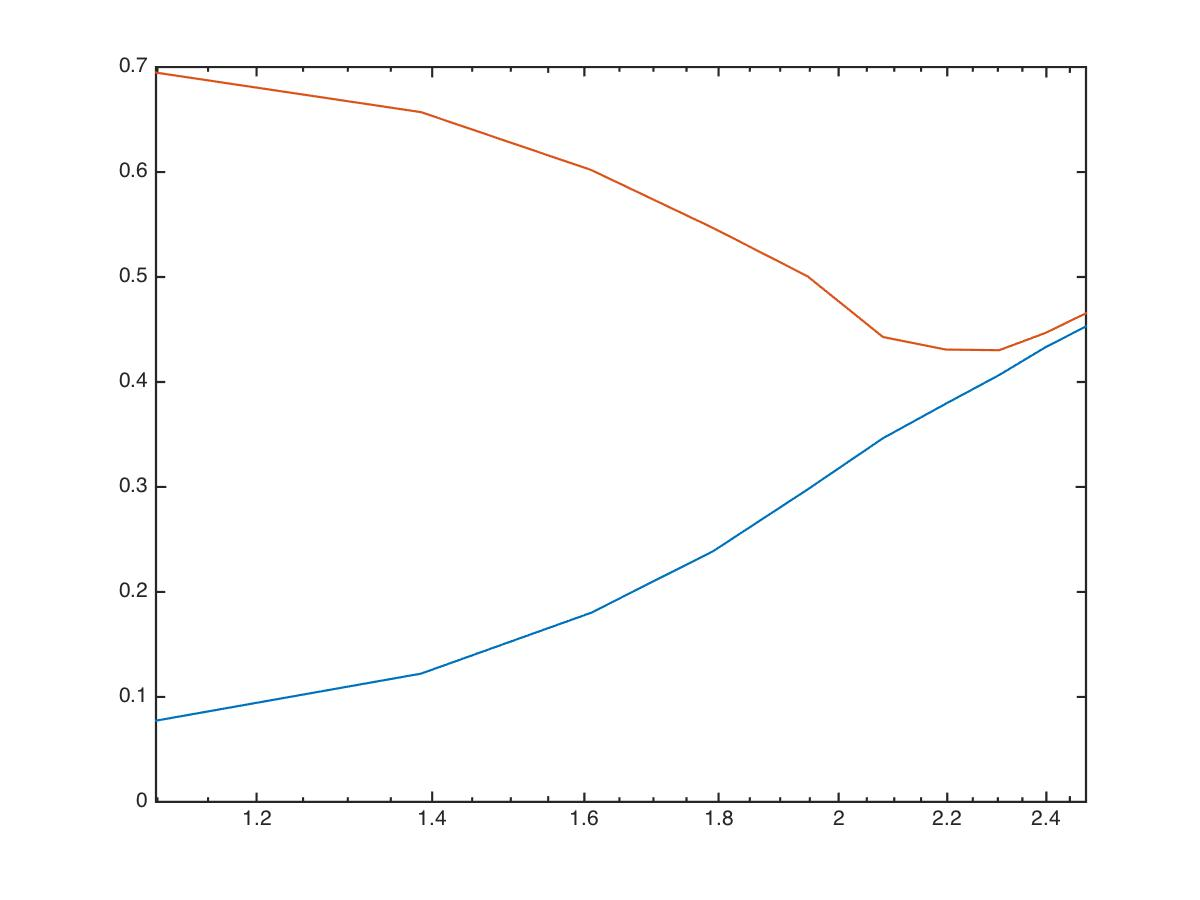
\includegraphics[scale=0.25]{minParent.jpg}
\caption[]{Text Here}
\label{fig:lr2}
\end{figure}

\begin{lstlisting}[caption={Plotting the scatter plot},label={lst:scatter},numbers=left,escapeinside={@}{@}]
\end{lstlisting}

\fi